\documentclass{ltjsarticle}

\usepackage{amsmath}
\usepackage{amssymb}
\usepackage{amsthm}
\usepackage{ mathrsfs }
\usepackage{enumerate}
\usepackage{bbm}
\usepackage{lipsum}
\usepackage{fancyhdr}
\usepackage{tikz-cd} 
\usetikzlibrary{graphs}
\usepackage{luatexja-ruby} 
\usepackage{graphicx} 
\graphicspath{ {./images/} }

\newtheorem{theorem}{定理}[section] 
\newtheorem{proposition}{Proposition}[section] 
\newtheorem{definition}{定義}[section] 
\newtheorem{problem}{問題}[section] 
\newtheorem{postulate}{公準}[section] 
\newtheorem{lemma}{Lemma}[section] 
\newtheorem{notation}{Notation}[section] 
\newtheorem{remark}{注釈}[section] 
\newtheorem{corollary}{系}[section] 
\newtheorem{terminology}{Terminology}[section] 
\newtheorem{example}{例題}[section] 
\newtheorem{step}{手順} 
\newtheorem{solution}{解答}[section] 
\newtheorem{fact}{事実}[section] 


\DeclareMathOperator{\diam}{diam}
\DeclareMathOperator{\Gal}{Gal}
\DeclareMathOperator{\rank}{rank}
\DeclareMathOperator{\Hom}{Hom}
\DeclareMathOperator{\Dom}{Dom}
\DeclareMathOperator{\Ann}{Ann}
\DeclareMathOperator{\grad}{grad}
\DeclareMathOperator{\Span}{Span}
\DeclareMathOperator{\interior}{int}
\DeclareMathOperator{\ind}{ind}
\DeclareMathOperator{\supp}{supp}
\DeclareMathOperator{\ob}{ob}
\DeclareMathOperator{\Spec}{Spec}
\DeclareMathOperator{\MaxSpec}{MaxSpec}
\DeclareMathOperator{\PreSh}{PreSh}
\DeclareMathOperator{\Sh}{Sh}
\DeclareMathOperator{\Fun}{Fun}
\DeclareMathOperator{\Ext}{Ext}
\DeclareMathOperator{\Aut}{Aut}
\DeclareMathOperator{\Ker}{Ker}
\DeclareMathOperator{\Image}{Im}
\DeclareMathOperator{\Coker}{Coker}
\DeclareMathOperator{\id}{id}
\DeclareMathOperator{\Mod}{Mod}
\DeclareMathOperator{\QCoh}{QCoh}
\DeclareMathOperator{\Coh}{Coh}
%\newcommand*{\name}[\num_arguments][default values]{{\color{#1}\Large #2}}
\newcommand*{\multivar}[2]{{#1_1,\cdots,#1_{#2}}}
\newcommand*{\localization}[2]{#1_{\mathfrak{#2}}}
\newcommand*{\ringedspacemorph}[1]{(#1,#1^{\#})}
\newcommand*{\sheaf}[2]{(#1,{\mathcal{#2}}_{#1})}
\newcommand{\fib}[1]{%
  \mathbin{\mathop{\times}\limits_{#1}}%
}
\newcommand{\tens}[1]{%
  \mathbin{\mathop{\otimes}\displaylimits_{#1}}%
}
\title{ボン補習校高校数学}
\author{}
\date{}

\begin{document}

\maketitle

\section{基礎情報}

\par\textbf{前提知識} : 中学３年生までの数学があれば十分です。
\par\textbf{授業について} 
\begin{enumerate}[	$\bullet$]
\item 毎週授業に出られない生徒のために板書と演習問題、その解答を載せた授業ノートをアップロードします。
\item 毎授業問題演習の時間を設けます。
\item 最初はそれぞれの生徒の数学の学習進度を確認します。
\end{enumerate}

\section{予定している単元一覧}

授業は次の四つの単元の内いくつかを選んでおこうなう予定です。気になる別の分野や、やってみたい問題などの希望が出た場合、単元の追加及び変更も予定しています。
\begin{enumerate}
\item \ltjruby{微分積分}{びぶんせきぶん}
\item \ltjruby{整数論}{せいすうろん}
\item グラフ理論
\item 平面図形
\end{enumerate}

とくに「\ltjruby{微分積分}{びぶんせきぶん}」と「平面図形」はAbiturの内容とも重なるところが多く、希望によってはAbiturの過去問の演習なども予定しています。

\subsection{\ltjruby{微分積分}{びぶんせきぶん}}

日本の高校のカリキュラムに習いつつ、大学の初年度の内容までの簡単な入門をすることを予定しています。とくに次のトピックについて授業をする予定です。
\begin{enumerate}[$\bullet$]
\item \ltjruby{微分}{びぶん}と\ltjruby{積分}{せきぶん}
\item 物理への応用
\item \ltjruby{線形代数}{せんけいだいすう}(Liniare Algebra)との関わり。
\end{enumerate}

例えば、高校で習う物理の公式として、あるものを静かに地面に落としたときのことを考えます。ここで
\begin{enumerate}
\item $t$ : 落としてからたった時間(秒)
\item $v(t)$ : $t$秒たったときのものが落ちている速度($m/s$)
\item $m$ : 物の\ltjruby{質量}{しつりょう}(kg)
\item $g$ : 地球の重力($m/s^2$)
\item $k$ : 物の形によって決まる\ltjruby{空気抵抗}{くうきていこう}の\ltjruby{係数}{けいすう}
\end{enumerate}
とすると、これは

\begin{equation*}
\begin{cases}
{\frac {dv} {dt}} = g-{\frac {kv} m}\\
v(0) = 0
\end{cases}
\end{equation*}
という式でかけます。最初の式は時間$t$によってどのように速度$v$が変化していくのか表しています。そして二番目の式は初めの状態を示しています。より正確にいうと、
\begin{enumerate}[$\bullet$]
\item 落ちている時間が長いほど落ちるスピードが上がる。
\item 落ちるスピードが速いほど\ltjruby{空気抵抗}{くうきていこう}も上がる。
\item 最初はスピードが$0$、つまり止まっている状態からスタートする。
\end{enumerate}
この式を解くと、
\begin{equation*}
v(t) = {\frac {mg} k}(1-e^{-{\frac k m}t})
\end{equation*}

となります。このような物理学においてよくでてくる式を解けることを一つの目標として授業を進めたいと考えています。
\par 高校よりも少し先の分野を紹介することで、教科書に突然現れる単元、例えば\ltjruby{自然対数}{しぜんたいすう}の\ltjruby{底}{てい}$e$や\ltjruby{行列}{ぎょうれつ}がなぜ必要なのかをわかりやすく伝えられるようにカリキュラムを作る予定です。


\subsection{\ltjruby{整数論}{せいすうろん}}

\ltjruby{整数論}{せいすうろん}は$1,2,3,4,\cdots$のような整数を勉強する分野です。この分野を勉強するための方法として余りのある割り算がよく使われます。$10$を$4$で割った余りが$2$であると言うのを
\begin{equation*}
10\equiv 2\mod{4}
\end{equation*}
と書いたりします。これは$10$と$2$は$4$で割った時の余りが同じであると言う意味でも使われます。なので、
\begin{equation*}
10\equiv 6\mod{4}
\end{equation*}
も成り立ちます。中学で勉強した\ltjruby{有理数}{ゆうりすう}を覚えていますか、たとえば
\begin{equation*}
{\frac 1 6}=0.16666\cdots
\end{equation*}
のようにパターン($6$がずっと続いている)のある少数(\ltjruby{循環小数}{じゅんかんしょうすう})は全て分数の形にできることを学びました。余りのある割り算を使うと次のことが証明できます。

\begin{theorem}
すべての\ltjruby{有理数}{ゆうりすう}は\ltjruby{循環小数}{じゅんかんしょうすう}として表せる。
\end{theorem}

\ltjruby{整数論}{せいすうろん}}を学ぶ場合はこの証明をゴールとしたカリキュラムを作ります。
\par 整数だけでなくあまりのある割り算は多項式のときにも便利です。例えば下の
\begin{equation*}
3x^2+x-5 
\end{equation*}
を$x$で割った余りは$-5$ですなぜなら、
\begin{equation*}
3x^2+x-5 = x(3x+1)-5
\end{equation*}
として書けるからです。もう一つのゴールとして、\ltjruby{虚数}{きょすう}$i$の存在を証明することもできます。すでに習った人も習っていない人もいるとおもいますが\ltjruby{虚数}{きょすう}とは
\begin{equation*}
i^2 = -1
\end{equation*}
となるような数です。皆さんが習ってきた実数は二乗すると$0$以上の数になります。なので\ltjruby{虚数}{きょすう}というのは全く新しい数なのです。多項式についてあまりのある割り算を考えると、この虚数を実際に作り出すことができます。
\par \ltjruby{整数論}{せいすうろん}}は他の単元と違い\ltjruby{抽象度}{ちゅうしょうど}が高い分野です。最初は慣れないと思いますが、みなさんが数学という学問をより広い\ltjruby{視野}{しや}}で捉えられるようになるカリキュラムを作る予定です。
\subsection{グラフ理論}

中学数学を習った皆さんがグラフと聞くと

\begin{center}
\begin{tikzpicture}
\draw[->] (-1.5,0)--(1.5,0) node[right]{$x$};
\draw[->] (0,-1.5)--(0,1.5) node[above]{$y$};
\draw[black]   plot[smooth,domain=-1:1] (\x, {\x*\x});
\end{tikzpicture}
\end{center}
のような $xy$座標のグラフを思い浮かべると思います。しかし、グラフ理論におけるグラフはこれとは大きく異なります。
\par グラフ理論におけるグラフとは次のような$A,B,C,D$と名前がつけられている点の関係性を線で表したものです。

\begin{center}
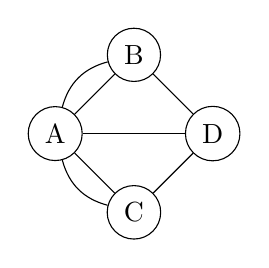
\begin{tikzpicture}[nodes={draw, circle}]
	\node (a) at (0,0) {A};
	\node (b) at (1,1) {B};
	\node (c) at (1,-1) {C};
	\node (d) at (2,0) {D};
\graph{
    (a)--(b)--(d);
    (a)--(c)--(d);
    (a)--(d);
    (a)--[bend left] (b);
     (a)--[bend right] (c);
};
\end{tikzpicture}
\end{center}
グラフ理論を使うと次のような定理を証明することができます。

\begin{theorem}[オイラーグラフの定理]
田んぼの「田」を一筆で描き切ることはできない。
\end{theorem}
\begin{theorem}[オイラーの\ltjruby{多面体}{ためんたい}定理]
それぞれの面が\ltjruby{正多角形}{せいたかっけい}となる立体はつぎの５種類のみである。
\begin{center}
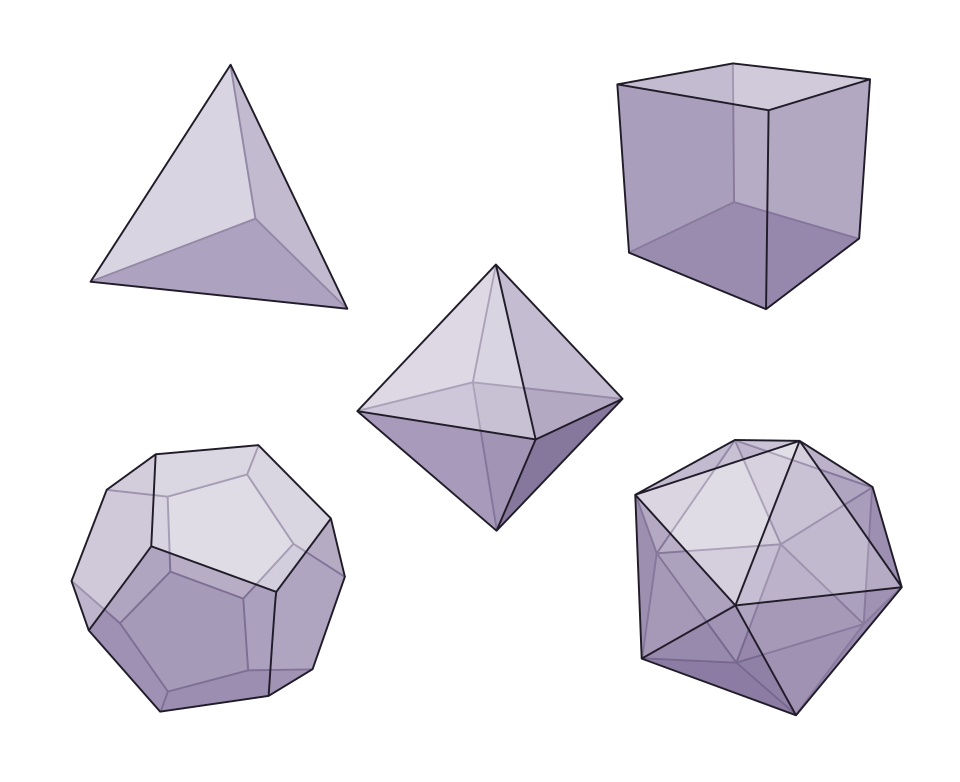
\includegraphics[scale=0.2]{platonicsolid}
\end{center}
\end{theorem}

\begin{theorem}[５色問題]
最低５種類の色があればどんな時代の地図もそれぞれ隣り合う国同士が違う色になるように塗ることができる。
\begin{center}
\begin{figure}[h]
	\centering
    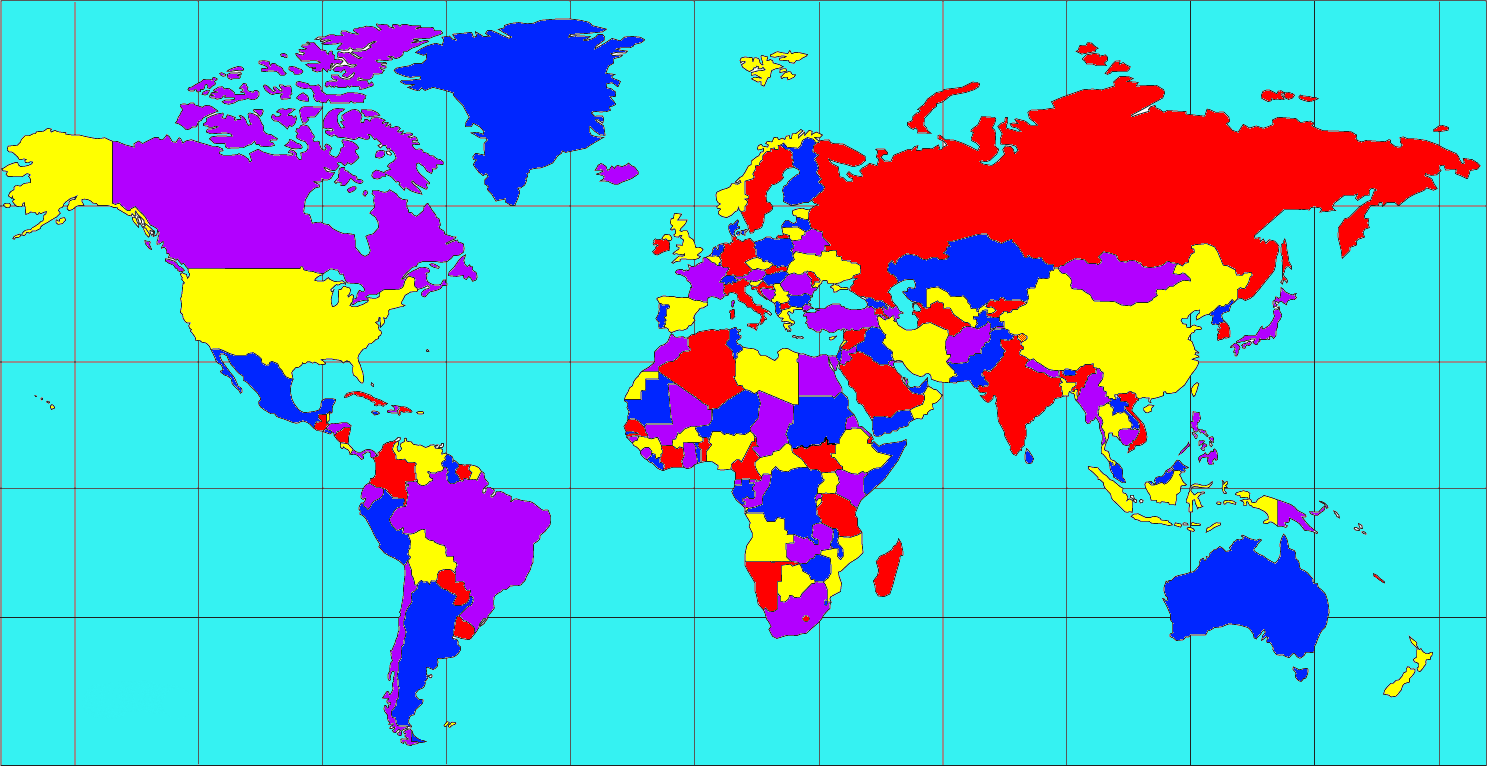
\includegraphics[scale=0.2]{world_map_five}
    \caption{赤青黄紫水色の5色で塗られた世界地図}
    \medskip
\small
くっついている国同士が違う色になっていることが確認できます。過去にはボンやケルンがローマ帝国の一部だったように、未来では国の形が変わるかもしれません。しかし、５色あればどんな時代の地図でもくっついている国同士が違う色になるように塗ることができます。
    \label{fig:my_label}
\end{figure}
\end{center}
\end{theorem}

さて、最初の図形に戻りましょう。

\begin{center}
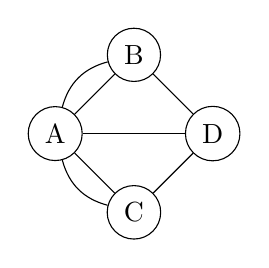
\begin{tikzpicture}[nodes={draw, circle}]
	\node (a) at (0,0) {A};
	\node (b) at (1,1) {B};
	\node (c) at (1,-1) {C};
	\node (d) at (2,0) {D};
\graph{
    (a)--(b)--(d);
    (a)--(c)--(d);
    (a)--(d);
    (a)--[bend left] (b);
     (a)--[bend right] (c);
};
\end{tikzpicture}
\end{center}

$A,B,C,D$と名前がつけられている丸を頂点といい、それらをつなぐ線は辺と呼ばれます。それぞれの頂点において、繋がっている辺の数をその頂点の\ltjruby{次数}{じすう}といいます。たとえば、$A$から出ている線は$5$つあります。よって$A$の\ltjruby{次数}{じすう}は$5$となります。$A$の\ltjruby{次数}{じすう}は記号を使って$d(A)$と書きます。これを使うと前の文章は
\begin{equation}
d(A) = 5
\end{equation}
と書けます。次数ついて次の定理が成り立ちます。

\begin{theorem}[\ltjruby{握手}{あくしゅ}の定理]$\:$
それぞれの頂点の\ltjruby{次数}{じすう}を足すと辺の数の二倍となる。
\end{theorem}
上の図だと
\begin{equation}
d(A)=5,\:d(B) = 3,\:d(C) = 3,\:d(D) = 3
\end{equation}
となるのでその和は
\begin{equation}
5+3+3+3 = 14
\end{equation}
となります。また辺の数は$7$個あるのでちょうど二倍になっていることがわかります。この定理の証明をしてみましょう。
\begin{proof}[証明]
辺を全て消した上のグラフを考えます
\begin{center}
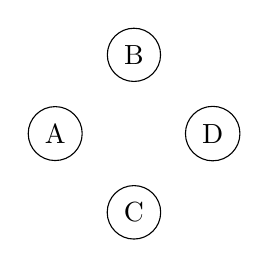
\begin{tikzpicture}[nodes={draw, circle}]
	\node (a) at (0,0) {A};
	\node (b) at (1,1) {B};
	\node (c) at (1,-1) {C};
	\node (d) at (2,0) {D};
\end{tikzpicture}
\end{center}
ここに一つ辺をつけると、
\begin{center}
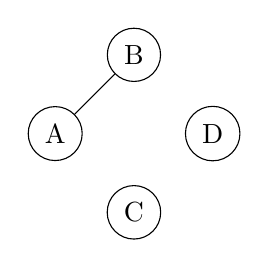
\begin{tikzpicture}[nodes={draw, circle}]
	\node (a) at (0,0) {A};
	\node (b) at (1,1) {B};
	\node (c) at (1,-1) {C};
	\node (d) at (2,0) {D};
\graph{
    (a)--(b);
};
\end{tikzpicture}
\end{center}
辺を一つ足すことで$A$と$B$の\ltjruby{次数}{じすう}がそれぞれ$1$ずつ増えました。よって\ltjruby{次数}{じすう}の合計は$2$ふえます。このように辺を一つ足すごとに\ltjruby{次数}{じすう}の合計は$2$ずつ増えるので、定理が成り立ちます。
\end{proof}
またグラフ理論はコンピューターサイエンスで活用されていて、とくに皆さんが常日頃使っているスマホのアプリなどの容量を減らす方法や動作を早くするための\ltjruby{基礎理論}{きそりろん}}などに役立っています。コンピューター系の分野に将来進みたい人は避けては通れない分野です。
\par \ltjruby{握手}{あくしゅ}の定理の証明のように、\ltjruby{直感的}{ちょっかんてき}で計算よりも考え方やアイデアが重要となってくる証明が多くあります。証明問題に対する苦手意識を持っている人などが、証明問題を好きになれるようなカリキュラムを作る予定です。
\subsection{平面図形}

平面図形の単元に関しては日本の高校教育のカリキュラムに習う予定です。具体的には、
\begin{enumerate}[$\bullet$]
\item 三角形の五心
\item チェバ・メネラウスの定理
\item 方べきの定理
\item ベクトルと三角比($\sin,\cos,\tan$)を使った\ltjruby{解析幾何}{かいせききか}(Analytische Geometrie)
\end{enumerate}
の学習を予定しています。以下のような証明問題を演習として解く予定です。

\begin{theorem}[フランク・モーリーの定理]
次のように角の三等分線を引くと、三角形の中央に正三角形$\triangle PQR$があらわれる。
\begin{center}
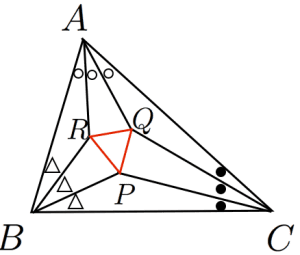
\includegraphics[scale=0.4]{morrey}
\end{center}
\end{theorem}

\begin{theorem}[オイラー線]
$H,G,O$をそれぞれ三角形$\triangle ABC$の\ltjruby{垂心}{すいしん}}、\ltjruby{重心}{じゅうしん}}、\ltjruby{外心}{がいしん}}とするとこれらがちょうど乗る一つの線がある。
\begin{center}
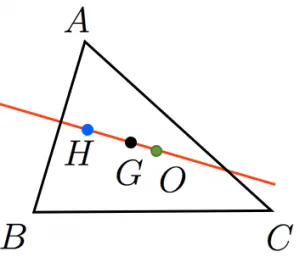
\includegraphics[scale=0.4]{euler_line}
\end{center}
\end{theorem}

上の二つの定理は、三角比をつかって\ltjruby{機械的}{きかいてき}に証明することもできれば、アイデア一つで面倒臭い計算をせずに証明することもできます。
\par 上のような美しい数学の定理と、エレガントな近道を探す証明の楽しさをメインに伝えられるような授業にする予定です。


%微分積分は物理学から生まれた数学です。この宇宙に比べて人間の目はとても小さく、全てを見通すには全くもって不十分です。しかし私たちは目の前に起こる小さな変化を観察することができます。そのような変化からなんとか世界の仕組みを知るために微分と積分は発明されました。おおざっぱにいうと微分とはその小さな変化を数式で書くための道具であり、積分はその変化の結果を知るための道具であると考えられます。
% \begin{center}
% \begin{tikzpicture}
% \draw[->] (-1.5,0)--(1.5,0) node[right]{$x$};
% \draw[->] (0,-1.5)--(0,1.5) node[above]{$y$};
% \draw[black]   plot[smooth,domain=-1.15:1.15] (\x, {\x*\x*\x});
% \draw(-0.8,-0.85)--(1.25,0.6875);
% \node at (0.5,0.125) [above]{P};
% \end{tikzpicture}
% \end{center}

% 微分をもう少し正確に説明すると上の図のように点$P$で曲線にぴったりくっつくような線を見つける計算方法のことを指します。また積分とは
% \begin{center}
% \begin{tikzpicture}
% \draw[->] (-1.5,0)--(1.5,0) node[right]{$x$};
% \draw[->] (0,-1.5)--(0,1.5) node[above]{$y$};
% \draw[black]   plot[smooth,domain=-1.15:1.15] (\x, {\x*\x*\x});
% \draw(1,0)--(1,1);
% \node at (0.8,0) [above]{S};
% \end{tikzpicture}
% \end{center}
% 積分とは曲線と縦線、そして$x$軸で囲まれている部分の面積を求める計算のことをいいます。この二つはそれぞれ足し算と引き算や掛け算と割り算のような対の関係になっています。
% \par 物理学において最も重要なことは\ltjruby{近似}{きんじ}です。近似とはニュートンがリンゴをボールとしたように、似ているものに置き換えて考える方法のことをいいます。この方法を数学的に書いたものを極限といいます。高校数学では多項式だけではなくさまざまな複雑な関数に出会うことになります。しかし極限を使うことにより、多項式によって近似できることを証明できます。たとえば
% \begin{equation}
% \sin(x) = x-{\frac 1 6}x^3+{\frac 1 {120}}x^5-\cdots
% \end{equation}
% 最終的には、かんたんな微分方程式を学習することを目標とします。例えば、空から落ちる物体を考えます。$m$を空から落ちる物体の重さ、$v$を落ちる速度、$g$を重力、$k$ある決まった数とします。空気抵抗を考えた落ちる物体の動きは
% \begin{equation}
% m{\frac {dv} {dt}} = mg-kv
% \end{equation}
% という式で表されれます。ここで$t$とは時間を表しています。物理だけでなく人口の増え方も微分方程式を使えば表せます。子供が生まれるには父親と母親が必要です。なので、ある街で子供が生まれる数はその街の人の数と関係しています。これを数学的に書くと
% \begin{equation}
% {\frac {dN} {dt}} = rN
% \end{equation}
% $N$は街にいる人の数、$r$は決まった数そして上と同じように$t$は時間を表します。空からまっすぐ降りてくる物体の式ですが、もちろん曲がった運動をする物体も微分方程式を使って書くことができます。
% \begin{equation}
% \begin{pmatrix}
% {\frac {dx} {dt}}\\ {\frac {dy} {dt}}
% \end{pmatrix}
% =\begin{pmatrix}
% -y\\x
% \end{pmatrix}
% \end{equation}
% はある点の周りを円を描くように回る物体の式です。微分積分を扱う場合は、このように数学を使って現実世界のことをどうやって表すことができるのかを目標に指導案を作ります。ドイツのAbiturの内容とかなさなる部分が多く「Lineare Algebra」や「Funktionen und Analysis」の発展的な内容となる予定です。

% \section{グラフ理論}

% 中学数学を習った皆さんがグラフと聞くと

% \begin{center}
% \begin{tikzpicture}
% \draw[->] (-1.5,0)--(1.5,0) node[right]{$x$};
% \draw[->] (0,-1.5)--(0,1.5) node[above]{$y$};
% \draw[black]   plot[smooth,domain=-1:1] (\x, {\x*\x});
% \end{tikzpicture}
% \end{center}
% のような $xy$座標のグラフを思い浮かべると思います。しかし、グラフ理論におけるグラフはこれとは大きく異なります。
% \par グラフ理論におけるグラフとは次のような$A,B,C,D$と名前がつけられている点の関係性を線で表したものです。

% \begin{center}
% \begin{tikzpicture}[nodes={draw, circle}]
% 	\node (a) at (0,0) {A};
% 	\node (b) at (1,1) {B};
% 	\node (c) at (1,-1) {C};
% 	\node (d) at (2,0) {D};
% \graph{
%     (a)--(b)--(d);
%     (a)--(c)--(d);
%     (a)--(d);
%     (a)--[bend left] (b);
%      (a)--[bend right] (c);
% };
% \end{tikzpicture}
% \end{center}
% グラフ理論を使うと次のような定理を証明することができます。

% \begin{theorem}[オイラーグラフの定理]
% 田んぼの「田」を一筆で描き切ることはできない。
% \end{theorem}

% \begin{theorem}[５色問題]
% 世界地図において、最低５種類の色があればそれぞれ隣り合う国同士が違う色になるように塗ることができる。
% \end{theorem}

% \begin{theorem}[オイラーの多面体定理]
% それぞれの面が正多角形となる立体はつぎの５種類のみである。
% \begin{center}
% 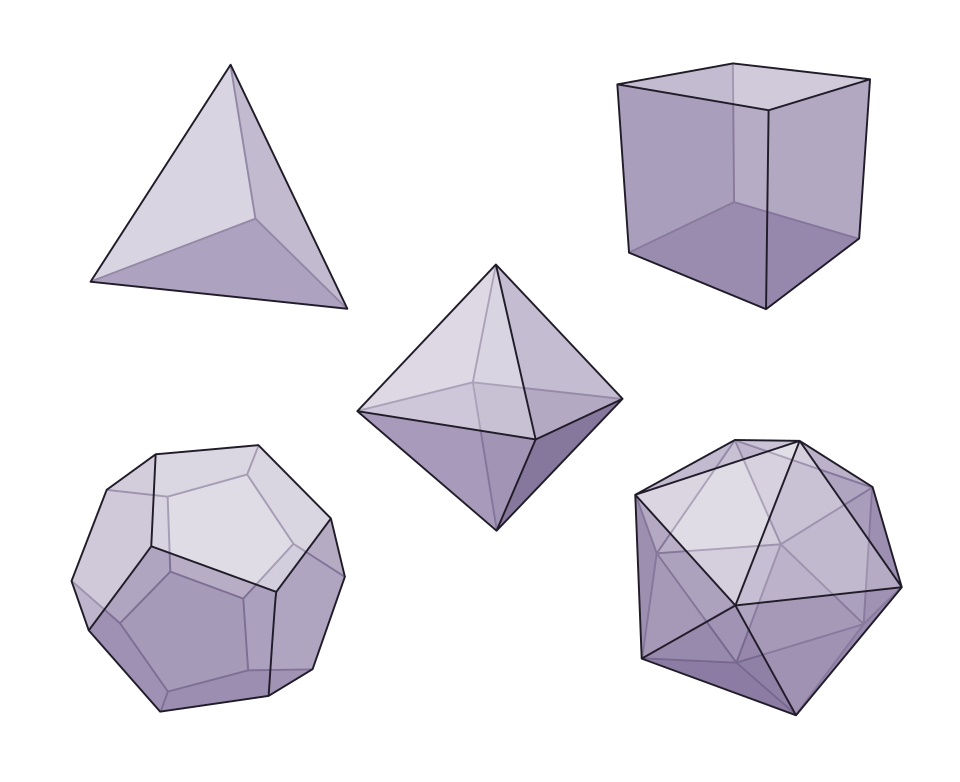
\includegraphics[scale=0.2]{platonicsolid}
% \end{center}
% \end{theorem}
% グラフ理論はコンピューターの分野で利用されていて、とくに皆さんが常日頃使っているスマホのアプリなどの容量を減らす方法や動作を早くするための基礎理論などに活用されています。さて、最初の図形に戻りましょう。

% \begin{center}
% \begin{tikzpicture}[nodes={draw, circle}]
% 	\node (a) at (0,0) {A};
% 	\node (b) at (1,1) {B};
% 	\node (c) at (1,-1) {C};
% 	\node (d) at (2,0) {D};
% \graph{
%     (a)--(b)--(d);
%     (a)--(c)--(d);
%     (a)--(d);
%     (a)--[bend left] (b);
%      (a)--[bend right] (c);
% };
% \end{tikzpicture}
% \end{center}

% $A,B,C,D$と名前がつけられている丸を頂点といい、それらをつなぐ線は辺と呼ばれます。それぞれの頂点において、繋がっている辺の数をその頂点の次数といいます。たとえば、$A$から出ている線は$5$つあります。よって$A$の次数は$5$となります。$A$の次数は記号を使って$d(A)$と書きます。これを使うと前の文章は
% \begin{equation}
% d(A) = 5
% \end{equation}
% と書けます。次数ついて次の定理が成り立ちます。

% \begin{theorem}[握手の定理]$\:$
% それぞれの頂点の次数を足すと辺の数の二倍となる。
% \end{theorem}
% 上の図だと
% \begin{equation}
% d(A)=5,\:d(B) = 3,\:d(C) = 3,\:d(D) = 3
% \end{equation}
% となるのでその和は
% \begin{equation}
% 5+3+3+3 = 14
% \end{equation}
% となります。また辺の数は$7$個あるのでちょうど二倍になっていることがわかります。この定理の証明をしてみましょう。
% \begin{proof}[証明]
% 辺を全て消した上のグラフを考えます
% \begin{center}
% \begin{tikzpicture}[nodes={draw, circle}]
% 	\node (a) at (0,0) {A};
% 	\node (b) at (1,1) {B};
% 	\node (c) at (1,-1) {C};
% 	\node (d) at (2,0) {D};
% \end{tikzpicture}
% \end{center}
% ここに一つ辺をつけると、
% \begin{center}
% \begin{tikzpicture}[nodes={draw, circle}]
% 	\node (a) at (0,0) {A};
% 	\node (b) at (1,1) {B};
% 	\node (c) at (1,-1) {C};
% 	\node (d) at (2,0) {D};
% \graph{
%     (a)--(b);
% };
% \end{tikzpicture}
% \end{center}
% 辺を一つ足すことで$A$と$B$の次数がそれぞれ$1$ずつ増えました。よって次数の合計は$2$ふえます。このように辺を一つ足すごとに字数の合計は$2$ずつ増えるので、定理が成り立ちます。
% \end{proof}

% \section{整数論}

% \ltjruby{整数論}{せいすうろん}とは書いてある通り整数に関する数学の分野です。たとえば、約数や素数などのことを考えます。
% \begin{example}
% 次の式が成り立つような二つの整数のペア$(x,y)$は存在するか。
% \begin{equation*}
% 2x+3y = 1
% \end{equation*}
% \end{example}
% \begin{proof}[解答]
% $x=-1$、$y=1$のときに成り立つ。
% \end{proof}

% 上の場合は$2$と$3$の差が$1$なので簡単に溶けましたが次の場合はどうでしょうか。
% \begin{example}
% 次の式が成り立つような二つの整数のペア$(x,y)$は存在するか。
% \begin{equation*}
% 53x+17y = 1
% \end{equation*}
% \label{example_euclide_difficult}
% \end{example}
% この式は$x=-8$、$y=25$の時に成り立ちます。これはユークリッドの\ltjruby{互除法}{ごじょほう}と呼ばれる世界で最も古いアルゴリズムを使って解くことができます。

% \begin{theorem}[ユークリッドの\ltjruby{互除法}{ごじょほう}]$\:$二つの正の整数$a$、$b$を考える。$a$が$b$よりも大きい時、$a$を$b$で割った時のあまり$r$について次のことが成り立つ。
% \begin{equation*}
% \text{$a$と$b$の最大公約数は$b$と$r$の最大公約数と同じ}
% \end{equation*}
% \end{theorem}

% \begin{proof}[例題\ref{example_euclide_difficult}の解答]
% \begin{align*}
% 53 &= 3\times 17+2\\
% 17 & = 8\times 2+1
% \end{align*}
% と書けるのでそれぞれの式を変形して、
% \begin{align*}
% 53-3\times 17 &= 2\\
% 17 -8\times 2& = 1
% \end{align*}
% 一つ目の式を二つ目に代入して
% \begin{equation}
% 17 - 8(53-3\times 7 ) = 1
% \end{equation}
% 展開して整理すると、
% \begin{equation}
% 25\times 17 - 8\times 53 = 1
% \end{equation}
% \end{proof}

% 二つの整数$a$と$b$をある整数$n$で割った時の余りが同じ時、
% \begin{equation}
% a\equiv b\mod{n}
% \end{equation}
% というふうに書きます。中学一年生で習った「互いに素」という言葉を覚えていますか。二つの数$a$と$b$が互いに素とは二つの最大公約数が$1$のことをいいます。
% \begin{theorem}[オイラーフェルマーの定理]
% $a$と$b$を互いに素な二つの整数とする。ある整数$e$が存在して
% \begin{equation}
% a^e\equiv 1\mod{b}
% \end{equation}
% となる。つまり$a^e$を$b$で割った余りが$1$となるような$e$が存在する。
% \end{theorem}

% \begin{example}
% \begin{align*}
% 3\equiv 3\mod{10}\\
% 9\equiv 9\mod{10}\\
% 27\equiv 7\mod{10}\\
% 81\equiv 1\mod{10}\\
% \end{align*}
% よって$a=3$、$b=10$とのき$e=4$となるとうまくいく。これを使って$3^{100}$を$10$で割った時の余りを計算せよ。
% \end{example}
% \begin{proof}[Solution.]
% $3^{100} = (3^4)^{25}$よって余りは$1$。
% \end{proof}

% この余りを考える計算は整数だけでなく多項式にも応用できます。例えば多項式を$x^2+1$で割った時の余りを考えてみましょう。
% \begin{equation*}
% ax^2+bx+c = a(x^2+1)+bx+(c-a)
% \end{equation*}
% のように書くことができます。よって二次の多項式を$x^2+1$で割った時の余りは$\alpha x+\beta$のような形で書けます。ここで$x^2$の余りを計算してみましょう、これは
% \begin{equation}
% x^2 = (x^2+1)-1
% \end{equation}
% と書くことができます。よって$x^2$と$-1$は$x^2+1$を法として合同となります。少し乱暴ですが通常のイコールとしてこれらを考えると$x$は二乗すると$-1$となります。\ltjruby{虚数}{きょすう}という\ltjruby{概念}{がいねん}を高校では習いますがこれは英語では「Imaginary Number（想像上の数）」と呼ばれるほどつかみどころのない数と思われていますが、実は余りを考えることにより実際に作り出すことができるのです。

% %このように余りのある割り算を考えるとうまくいく問題があります。また最大公約数ではなくあまりそのものを考えることで見通しが良くなる場合もあります。$2$で割り切れる数を偶数、そうでない数を奇数と呼びますが、この二つについて次のことが成り立ちます
% %\begin{equation}
% %\text{偶数}+\text{偶数}=\text{偶数},\:\text{偶数}+\text{奇数}=\text{奇数},\text{奇数}+\text{奇数}=\text{偶数}\label{equation_sum_mod_2}
% %\end{equation}
% %また掛け算についても
% %\begin{equation}
% %\text{偶数}\times\text{偶数}=\text{偶数},\:\text{偶数}\times\text{奇数}=\text{偶数},\text{奇数}\times\text{奇数}=\text{奇数}\label{equation_product_mod_2}
% %\end{equation}
% %このことを$2$で割り切れるかどうかだけではなくさまざな数の割り算に応用できないでしょうか。$2$で割った時の余りは$0$か$1$です。$0$の時は偶数、$1$の時は奇数となります。記号を使ってこれを書く方法を考えます。ある整数$n$について、$2$で割った時の余りが$0$、$1$のときをそれぞれ
% %\begin{equation}
% %n\equiv0\mod{2},\quad n\equiv1\mod{2}
% %\end{equation}
% %と書きます。$\mod$とは英語で余りを意味する「modulo」の略。$\equiv$は$=$と区別するために使われています。これを使って式\eqref{equation_sum_mod_2}と式\eqref{equation_product_mod_2}を書き直すと
% %\begin{equation}
% %0+0\equiv0\mod{2},0+1\equiv 1\mod{2},1+1\equiv0\mod{2}
% %\end{equation}
% %また
% %\begin{equation}
% %0\times0\equiv0\mod{2},0\times 1\equiv0\mod{2},1\times 1\equiv1\mod{2}
% %\end{equation}

% %と書けます。

% \section{幾何学}
% \subsection{合同変換}

% 関数の定義を覚えていますか。関数$f$とはある$x$を決めるとただ一つの$f(x)=y$が決まる関係のことでした。これは何かのインプットに対してアウトプットがうまく決まるような関係ともいえます。この$x$と$y$どちらも数字の場合をずっと中学数学で習っていました。少しこの考えを拡張してみましょう。
% \begin{center}
% \begin{tikzpicture}
% \draw (-0.5,0)node[below]{A}--(-2,0)node[left]{B}--(-1,0.75)node[above]{C}--cycle;
% \draw (0.5,0)node[below]{A'}--(2,0)node[right]{B'}--(1,0.75)node[above]{C'}--cycle;
% \draw (0,-1)node[left]{$l$} -- (0,1.5);
% \end{tikzpicture}
% \end{center}

% たとえばある点$A$インプットとし、線$l$を対称の軸として線対称な点$A'$へアウトプットする関係を$T$とすると、上のように$\triangle ABC$の上にある点は$T$によって$\triangle A'B'C'$の上の線対称な点へと移動されます。二つの三角形は線対称なので合同です。このように、どんな三角形をインプットしてもそれと合同な三角形がアウトプットされる関数を合同変換と言います。上の図の合同変換のことを鏡映とよび、次の意味で最も重要な合同変換だといえます。

% \begin{theorem}
% どんな合同変換も多くても三つの鏡映の組み合わせで表すことができる。
% \end{theorem}

% 三角形とは三つの点とそれらをつなぐ三つの直線分でできています。三角形が別の合同な三角形にアウトプットされることから、まっすぐな線はこの関数によってまっすぐな線にアウトプットされることがわかります。
% このようにまっすぐなものをまっすぐなものにアウトプットする変換のことを線形変換と呼びます。

% \subsection{非ユークリッド幾何学}
% 数学には\ltjruby{公理}{こうり}と呼ばれる最も基本的なルールが存在します。ルールを互いに矛盾しないように定めることにより様々な数学の分野を作ることができるのです。とくに平面幾何の場合は次の五つが定められています。

% \begin{enumerate}[公理 I : ]
% \item ある二つの点の間をむすぶ直線を引くことができる。
% \item ある直線の片側を無限にまっすぐ伸ばすことができる。
% \item ある長さと点があるときに、その点を中心、長さを半径とした円を描くことができる。
% \item すべての直角の大きさは等しい。
% \item 線とその上にない点があるとき、その点を通って与えられた線に並行な直線はただ一つ存在する。
% \end{enumerate}

% 五番目の公理は平行線公理とよばれ、前の四つに比べて少し複雑なことからより単純なものにできないか、もしくは前の四つをつかって証明できないかどうか長い間議論されていました。１９世紀になり、ロシアのロバチェフスキー、ハンガリーのボヤイ、そしてドイツのガウスがそれぞれ独自に四つを使って証明することが不可能であることを示しました。つまり、この公理を取り除いた場合、新しい二つの数学の分野である「\ltjruby{双曲幾何学}{そうきょくきかがく}」と「\ltjruby{球面幾何学}{きゅうめんきかがく}」が誕生することがわかったのです。
% \begin{figure}[h]
% 	\centering
%     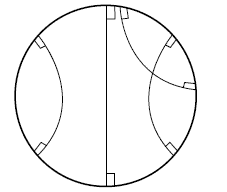
\includegraphics[width=0.28\textwidth]{poincare_disk_model}
%     \caption{双曲幾何のモデル（ポアンカレディスク}
%     \medskip
% \small
% 双曲幾何ではこのように曲がった線が直線となる。\\ また五番目の公理の「ただ一つ存在する」が「無数に存在する」に変わる。
%     \label{fig:my_label}
% \end{figure}
% \begin{figure}[h]
% \centering
%     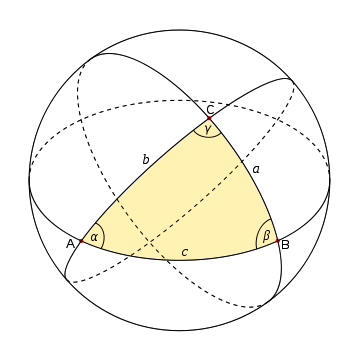
\includegraphics[width=0.28\textwidth]{spherical_triangle}
%     \caption{球面幾何の三角形}
%         \medskip
% \small
% 球面幾何の三角形は平面幾何のものと比べて少しふくらんでいて、内角の和は$180^\circ$を超える。\\ また五番目の公理の「ただ一つ存在する」が「存在しない」に変わる。
%     \label{fig:my_label}
% \end{figure}
% \par 特に双曲幾何は宇宙空間と密接に関係していて、アインシュタインの生み出した\ltjruby{一般相対性理論}{いっぱんそうたいせいりろん}は本質的には双曲幾何を現実世界に応用したものと言えます。また、ドイツの学校で習う「Analytische Geometrie」はこのような理論の最も簡単な場合を扱っていると言えるでしょう。 

\end{document}